\subsection*{a)}

A simple two-chemical model for a Belousov-Zhabotinsky reaction can be described by,

\begin{align}
\label{eq:2a}
\frac{\partial u}{\partial t}& = a - (b-1)u + u^2v + \nabla^2 u,\\
\frac{\partial v}{\partial t}& = bu - u^2v + D_v \nabla^2 v.
\end{align}

For a spatially homogeneous steady state the following conditions must hold,

$$0 = a - (b+1)u + u^2v$$
$$0 = bu - u^2v$$

The steady state 

$$
(u^*,v^*)
$$
is found through simple calculations. To find if the steady state is stable the Jacobian is first calculated
$$J^* = \left(
\begin{array}{cc}
    b-1 & a^2 \\
    -b  & -a^2
\end{array}
\right).$$

For the steady state to be stable the following conditions must be true

$$Tr(J^*) < 0$$
$$Det(J^*) > 0.$$

Inserting the given values $a=3$, $b=8$ the following results are produced
$$Tr(J^*) = -2 < 0$$
$$Det(J^*) = 9 > 0.$$
Thus the steady state is stable.

For the system to exhibit diffusion driven instability (DDI) the following conditions must also hold

$$D_v \frac{\partial f}{\partial u} + \frac{\partial g}{\partial v} < 0$$
$$(D_v \frac{\partial f}{\partial u}+ \frac{\partial g}{\partial v})^2 - 4D_v Det(J^*) > 0$$

Inserting the values for $a, b$ and $(u^*, v^*)$, the first equation gives rise to the condition on $D_v$,

$$D_v > \frac{9}{7}$$

and the second
$$D_v > \frac{81}{49} + \sqrt{\left(\frac{81}{49}\right)^2 - \frac{81}{49}} = 2.69$$
or
$$D_v < \frac{81}{49} - \sqrt{\left(\frac{81}{49}\right)^2 - \frac{81}{49}} = 0.61.$$

Thus for the system to exhibit diffusion driven instability $D_v > 2.69$, since $0.61 < \frac{9}{7}$.


\subsection*{b)}

In figure \ref{fig:pic2b} we see the result of simulating the following system described by \eqref{eq:2a} on a 128 by 128 lattice.

This is done using integration with a time step of $\Delta t = 0.01$ and also using a discretized Laplacian. Our Implementation uses four matrices, two that stores the previous state for both u and v in all positions, and two that are used for temporarily storing the state in each time step. This is done simply by having three for loops, one which takes care of the time steps and two that iterates through $x$ and $y$ of the matrices. At each time step one part of the integration is calculated.

\begin{figure}[h]
\centering
System Simulated with $D_v=2.3$\\
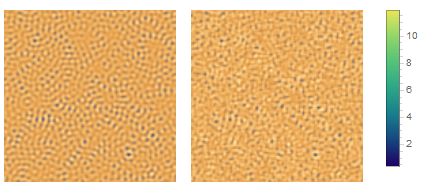
\includegraphics[scale=0.5]{img/2bd23Comb.png}\\
System Simulated with $D_v=3$\\
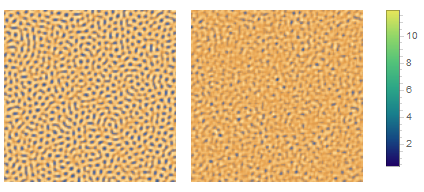
\includegraphics[scale=0.5]{img/2bd3Comb.png}\\
System Simulated with $D_v=5$\\
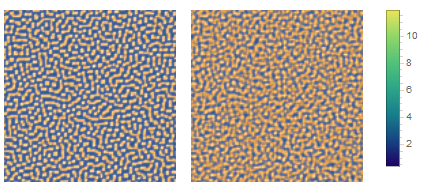
\includegraphics[scale=0.5]{img/2bd5Comb.png}\\
System Simulated with $D_v=9$\\
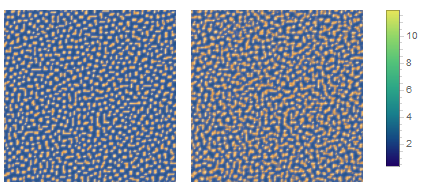
\includegraphics[scale=0.5]{img/2bd9Comb.png}\\
\caption{\label{fig:pic2b} The pictures to the left shows the system in the transient state after 200 time steps, for different values of $D_v$, and the pictures to the right shows the system after reaching the spatially inhomogeneous steady state.}
\end{figure}
